\thispagestyle{empty}
{\vrule height 0mm depth 30mm width 0mm}
\par
Mit dem Beginn der Arbeiten an der Reihe VIII der Akademie-Ausgabe G. W. Leibniz, \textit{S\"{a}mtliche Schriften und Briefe} wurden achtzig Jahre nach dem Erscheinen des 1. Bandes dieses Traditionsunternehmens die naturwissenschaft\-lichen, medizinischen und technischen Schriften von Gottfried Wilhelm Leibniz erstmals zum Gegenstand systematischer editorischer Bem\"{u}hungen. Der Rezeption des Leibniz'schen Oeuvre wird damit eine Dimension erschlossen, die in ihren Wirkungen weit \"{u}ber eine bloß werkgeschichtliche Bedeutung hinaus reicht. Heute nach wie vor pr\"{a}sente Resultate seiner naturwissenschaftlichen und technischen T\"{a}tigkeit wie die Rechenmaschine, die er auch schon als duale konzipierte und damit zum Stammvater des Computers wurde, das Maß der lebendigen Kraft und der Organismusbegriff sind Glanzpunkte eines Wissenschaftskonzepts, dessen methodologische Strategien und disziplin\"{a}re Auslegungen in der Reihe VIII ediert werden.\par
Damit erh\"{a}lt das inzwischen zunehmende Interesse der Forschung an Leibniz’ Arbeiten im Felde der Erfahrungswissenschaften seine ad\"{a}quate Quellenbasis. Und wie die bislang vorliegenden Ergebnisse zeigen, wird man das tradierte Dik\-tum von Leibniz als Repr\"{a}sentanten eines der großen rationalistischen Systeme des 17. Jahrhunderts, das in der Vergangenheit sowohl f\"{u}r die Quellenerschließung als auch f\"{u}r deren Deutung die Richtung vorgegeben hat, modifizieren m\"{u}ssen.\par
Dass Leibniz sp\"{a}testens seit seiner Ankunft in Paris im Fr\"{u}hjahr 1672 die empirischen Wissenschaften seiner Zeit nicht nur studiert, sondern wissenschafts\-theoretisch reflektiert hat, dass er eine eigene Wissenschaftsmethodologie ent\-wickelte, in der auch ein Experimentum crucis nicht fehlt, und dass er schließlich ein eigenes Physikkonzept ausarbeitete, das sich als Alternative zu Newton verstand und dar\"{u}ber hinaus auch noch die empirischen Wissenschaften als messende Wissenschaften stringent begr\"{u}ndete, dies alles wird sich anhand der Edition der Schriften der Reihe VIII studieren lassen. In welcher Weise davon auch das Verst\"{a}ndnis der Physik und ihrer Geschichte tangiert werden, wird sich im Detail zeigen m\"{u}ssen. Erste Versuche einer logischen Rekonstruktion der Entwicklung von Leibniz und Euler bis zur Relativit\"{a}tstheorie und Quantenmechanik\footnote{\footnotesize Vgl. P. Enders, \textit{Von der klassischen Physik zur Quantenphysik}, Berlin 2006 und D. Suisky, \textit{Euler as Physicist}, Berlin 2008.} lassen schon heute erkennen, dass die zu erschließenden Quellen keineswegs allein von historischem Interesse sein werden.\par
Der Band VIII, 1 gibt davon einen ersten Eindruck. Er umfasst insge\-samt 71 St\"{u}cke aus den Jahren 1668\textendash 1676, die sich um die Themenfelder Nautik, Optik, Pneumatik und Technik gruppieren. Ein St\"{u}ck hat, wie bereits aus dem Titel \textit{Observata philosophica} hervorgeht, \"{U}berblickscharakter. Es enth\"{a}lt ein Klassifikationssystem der Wissenschaften, das f\"{u}r Leibniz' Denken in dieser Zeit von orientierender Bedeutung ist und daher der Edition des ersten Bandes seiner naturwissenschaftlichen, medizinischen und technischen Schriften vorangestellt wird. Inhaltlich wird der vorliegende Band durch Studien zur Pneumatik dominiert. Sie beanspruchen etwa die H\"{a}lfte des Gesamtumfangs. Die \"{u}brigen Gegenstandsgebiete sind zu etwa gleichen Teilen in dem Band vertreten.\par
Wie in allen anderen Schriftenreihen, ist auch f\"{u}r die Reihe VIII eine chronologisch-systematische Pr\"{a}sentation der Texte das bestimmende Prinzip. Die in \textit{LSB} VIII, 1 publizierten Schriften reichen bis in die fr\"{u}he Zeit von Leibniz' Aufenthalt in Mainz (1667\textendash 1672) zur\"{u}ck und pr\"{a}sentieren in ihrer Mehrheit die geistigen Ergebnisse der wohl fruchtbarsten und wirkm\"{a}chtigsten Periode seiner intellektuellen Biografie, der Pariser Zeit von 1672 bis 1676.\par
Denselben Zeitraum wird der darauf folgende Band \textit{LSB} VIII, 2 umfassen, in dem die Schriften zur Astronomie und Mechanik, zur Botanik, Alchimie und Medizin publiziert werden. Auch f\"{u}r diesen Band ist die nat\"{u}rliche Z\"{a}sur der Abreise aus Paris mit dem anschlie{\ss}enden Dienstantritt in Hannover das Kriterium f\"{u}r die Auswahl der Texte. Beide B\"{a}nde bilden eine durch \"{u}bergreifende inhaltliche Fragestellungen und die Rahmenbedingungen der Pariser Zeit bestimmte Einheit.\par
Von den 71 St\"{u}cken des 1. Bandes der Reihe VIII ist allein der Text N.~14\textsubscript{2}, der in unserer Ausgabe 2 1/2 Druckseiten umfasst, bereits zu Leibniz' Lebzeiten publiziert worden. F\"{u}nf weitere Texte (N.~11, N.~13, N.~18, N.~22 und N.~58) mit einem Umfang von insgesamt 32 Druckseiten wurden sp\"{a}ter von Ernst Gerland (\textsc{Gerland} 1906) l\"{u}ckenhaft ediert. Im Druck zug\"{a}nglich sind auch N.~48\textsubscript{1} (10 Druck\-seiten)\footnote{\footnotesize M. L. Alcoba, \textit{G. W. Leibniz: Consequence de l'Hypothese generalle publi\'{e}e il y a quelque temps, pour expliquer le Phenomene de l'attachement dans le vuide, ou dans une place dont l'air a est\'{e} tir\'{e}}, in: \textit{Studia Leibnitiana} XXVIII (1996) S. 7\textendash 16.} sowie Fragmente\footnote{\footnotesize K. I. Gerhardt, \textit{Leibniz in London}, in: \textit{Sitzungsberichte der Preu{\ss}ischen Akademie der Wissenschaften} X (1891) S. 157\textendash 176, darin S. 165\textendash 166.} von N.~1. Alle anderen Konzepte, Notizen, Exzerpte, Ab- und Reinschriften sowie Marginalien werden mit dem vorliegenden Band der Forschung erstmals zur Verf\"{u}gung gestellt.\par
Von diesen Textzeugen hat Leibniz die St\"{u}cke N.~2, N.~53, N.~54, N.~58, und N.~68 selbst datiert. Drei Texte (N.~6\textsubscript{2}, N.~7 und N.~19) liegen als Abschriften vor, wobei Leibniz im Falle von N.~6\textsubscript{2} auch der Autor der Textvorlage ist. Die beiden anderen Abschriften wurden f\"{u}r ihn angefertigt. Bei einem einzigen Text (N.~67) handelt es sich um eine Reinschrift.\par
Einen relativ breiten Raum nehmen im vorliegenden Band die Annotationen sowie An- und Unterstreichungen in Marginalienexemplaren ein. Sie beziehen sich fast ausschlie{\ss}lich auf Druckschriften zur Optik.\par\vspace{2.0ex}

Das Editionskonzept\par\vspace{1.0ex}

Die Aufnahme der Daten f\"{u}r den Druck erfolgt in einer Weise, die dem Leser neue M\"{o}glichkeiten der Auseinandersetzung mit dem Text und dessen Entstehung er\"{o}ffnet. F\"{u}r die Reihe VIII wurden daf\"{u}r s\"{a}mtliche infrage kommenden Handschriften digitalisiert und in einem Umfang von etwa 45000 Scans in drei Aufl\"{o}sungen allen Interessenten weltweit online zur Verf\"{u}gung gestellt. Der Zugang zu diesen Handschriften erfolgt ohne Passwort und ist \"{u}ber den Online-Ritter-Katalog der Leibniz-Handschriften und -Briefe (http://ritter.bbaw.de) m\"{o}glich.\par
Zur Herstellung des Textes laden sich die Editoren die Bilddateien der Handschriften auf ihren Computer, transkribieren diese und senden die Arbeitsergebnisse (soweit es sich um außerhalb Berlins t\"{a}tige Mitarbeiter handelt) via Internet an die Berliner Arbeitsstelle der Leibniz-Edition, wo sie gegengelesen, redigiert und archiviert werden. Sobald eine Handschrift bearbeitet ist, wird sie mithilfe eines speziell entwickelten Programms, das die Dateien auf formale Korrektheit kontrolliert, hochgeladen und im Rahmen der Internetedition des im Entstehen begriffenen Bandes online pr\"{a}sentiert. Die Internetedition ist unter der Adresse http://leibnizviii.bbaw.de erreichbar und bildet den Ausgangspunkt f\"{u}r das Generieren der Druckfassung. Zu diesem Zweck wurde ein Konverter entwickelt, der die Daten der Internetedition so transformiert, dass die B\"{a}nde auf der Grundlage eines TEX-Skripts gesetzt werden k\"{o}nnen. Das Satzprogramm wurde unter Ver\-wendung des ledmac-packets geschrieben. Dem Erstellen des Druckmanuskripts geht damit eine Darstellungsform voraus, die als Internetedition die spezifischen Bedingungen des world wide web zur Textpr\"{a}sentation nutzt und so die erw\"{a}hnten neuen M\"{o}glichkeiten f\"{u}r den Leser schafft. Dies bedeutet unter anderem, dass sich jeder, der zuk\"{u}nftig einen Band der Reihe VIII aufschl\"{a}gt, wahlweise im Ritterkatalog oder in der Internetedition die zugeh\"{o}rige Handschrift auf seinem Computer aufrufen kann. Er kann diese in der Internetedition dem Zeilenfall des Originals folgend in einer Transkription vergleichen und durch bloßen Mausclick ein St\"{u}ck weit die Entstehung des Textes simulieren. Ein Leser der Akademie-Ausgabe, denn auf diese und nur auf diese ist die Internetedition \mbox{durch} die Auf\-nahme der Handschriftenpaginierung in das Druckmanuskript bezogen, kann, summarisch ausgedr\"{u}ckt, seine Lekt\"{u}re durch eine dynamische Pr\"{a}sentation erg\"{a}nzen und weitere M\"{o}glichkeiten des Internets wie die seitengenaue Verlinkung auf Referenzstellen nutzen, um sich etwa \"{u}ber eine Anspielung oder eine nur erw\"{a}hnte Zeichnung ins Bild zu setzen.\par
Diese Art der Herstellung und Pr\"{a}sentation der Texte schafft durch die Vergleichbarkeit von Original und Transkription eine neue Form von \"{O}ffentlichkeit, in der sich die Editoren bereits bei der Erstellung der Texte der \"{o}ffentlichen Kritik stellen und die Nutzer umgekehrt den Prozess der Textherstellung selbst mitgestalten k\"{o}nnen, und dies weltweit.\par\vspace{2.0ex}

Zum Inhalt\par\vspace{1.0ex}

Von den in der Zeit zwischen 1668 und 1676 entstandenen Texten mit natur\-wissenschaftlichem Inhalt ist ein Teil bereits in den B\"{a}nden 2 und 3 der Reihe VI der Akademie-Ausgabe erschienen. Darunter befinden sich sowohl Spezialuntersuchungen wie die Abhandlungen zur Optik in \textit{LSB} VI, 2 N.~46\textsubscript{1} \textendash\ N.~46\textsubscript{3} als auch Schriften vom Charakter der \cite{00256}\textit{Hypothesis physica nova} (\textit{LSB} VI, 2 N.~40), die eher einen allgemeineren Anspruch im Sinne der Naturphilosophie formulieren. An einigen Stellen des vorliegenden Bandes (z. B. N.~22 und N.~48) wird auf solche Schriften Bezug genommen. Sie markieren dort den theoretischen Ausgangspunkt f\"{u}r \"{U}berlegungen, die aufgrund bis dahin unbekannter experimenteller Erfahrungen neu zur intellektuellen Disposition gestellt werden.
Dieser Sachverhalt ist charakteristisch f\"{u}r die hier vorzustellenden Texte. Sie weisen im Vergleich mit den in der Akademie-Ausgabe bereits gedruckten eine Materialf\"{u}lle und Faktenbasis auf, die nicht nur neu, sondern im Falle der Pneumatica auch enorm ist. Bereits der erste Text unseres Bandes ist daf\"{u}r repr\"{a}sentativ.
Das St\"{u}ck ist nach Leibniz' erstem Besuch in London entstanden und, wie aus dem vollst\"{a}ndigen Titel \textit{Observata philosophica in itinere Anglicano sub initium anni 1673} hervorgeht, auf dem Wege von London zur\"{u}ck nach Paris niedergeschrieben worden. Es handelt sich um eine erste Systematisierung seiner Londoner Begegnungen und Erkenntnisse, die in der Form rubrizierter Schriften eine Art Klassifizierung der Wissenschaften nach Arithmetica, Geometrica, Musica, Optica, Astronomica, Mechanica, Pneumatica, Meteorologica, Hydrostatica, Magnetica, Nautica, Botanica, Anatomica, Chymica, Medica und Miscellanea bietet.\par
Die in diesem Zusammenhang aufgef\"{u}hrten Titel d\"{u}rften in der Regel f\"{u}r Leibniz neu gewesen sein. So erw\"{a}hnt er etwa in Bezug auf Boyle die gerade erschienenen \textit{Notae de atmosphaeris corporum consistentium} sowie die \textit{Exercitationes de atmosphaeris corporum consistentium}, nicht jedoch die ihm l\"{a}ngst bekannten \textit{New experiments physico-mechanical, touching the spring of the air}. Und in der Rubrik Optica wird erstmals Newton genannt, der bis dahin im Zusammenhang mit Problemen der Optik unerw\"{a}hnt blieb. 
Der Zuwachs an neuen Eindr\"{u}cken spiegelt sich auch in den Begegnungen wider, \"{u}ber die der Text indi\-rekt Auskunft gibt, indem er Notizen zu Ereignissen enth\"{a}lt, die sich auf Sitzungen der Royal Society zugetragen haben, an denen Leibniz entweder selbst teilgenommen hat oder \"{u}ber die er Informationen aus erster Hand besa{\ss}. Sie finden sich in den \textit{Observata philosophica} u. a. zur Botanik und Anatomie. Schlie{\ss}lich werden vor allem in den Rubriken Chymica und Miscellanea Kuriosit\"{a}ten notiert. Darunter der Hinweis auf eine Fornax multituba, auf eine neue Art von Metallen oder auf eine verloren gegangene Kunst des Emaillierens.\par
Die umfangreichsten Notizen entfallen auf Chymica und Medicina. Dies\-bez\"{u}glich herrscht dasselbe sammelnde Interesse vor, das man bereits von den fr\"{u}hen Akademieschriften her kennt, freilich um viele Details wie das Aus\-h\"{a}rten und Schmelzen von Metallen, um Rezepturen, Krankheiten und deren Heilungsmethoden sowie Medikamente bereichert.\par\vspace{2.0ex}

Nautik\par\vspace{1.0ex}

Die fr\"{u}hesten Texte unseres Bandes (N.~2\textsubscript{1} bis N.~2\textsubscript{5}) befassen sich mit dem im 17. Jahrhundert heftig debattierten und f\"{u}r die Schifffahrt au{\ss}erordentlich bedeutsamen Problem der L\"{a}ngengradbestimmung. Leibniz hat sie noch in Mainz verfasst und als Entstehungszeitraum Ende 1668 bis Anfang 1669 angegeben. Die Handschrift weist nur relativ wenige Korrekturen auf und fasst offenbar seinen Kenntnisstand der Materie in diesem Zeitraum zusammen.\par
Den Ausgangspunkt f\"{u}r die eigenen \"{U}berlegungen bildet Huygens' Darstellung der Benutzung von Pendeluhren f\"{u}r die Bestimmung der geographischen L\"{a}nge auf See. Leibniz rekapituliert dieses Verfahren und stellt dann sofort fest, dass selbst Huygens' Erfindung der Pendeluhr die Methode nicht vollkommen \mbox{macht}. Als Grund daf\"{u}r gibt er die Abh\"{a}ngigkeit von der Kenntnis der Orts\-zeit an, die durch Beobachtung der Sonne oder des Mondes ermittelt werden muss. Diese aber erweist sich als witterungsabh\"{a}ngig und ist folglich nicht immer verf\"{u}gbar.\par
Als L\"{o}sung des Problems skizziert Leibniz das Funktionsprinzip einer Maschine, die den Kurs eines Schiffes aufzeichnet, indem sie diesen automatisch auf eine Karte \"{u}bertr\"{a}gt. Er denkt dabei an einen Mechanismus, der in immer gleichen zeitlichen Abst\"{a}nden die Karte mit einer Nadel perforiert, so dass aus der Lage der L\"{o}cher die Rich\-tung und aus deren Abstand die Geschwindigkeit der Bewegung des Schiffes abgelesen werden k\"{o}nnen. Leibniz ist sich im Klaren dar\"{u}ber, dass seine Grundidee durch konstruktive Elemente praktikabel gemacht werden muss, die den Einfluss des Wassers und des Windes auf die Bewegung des Schiffes kompensieren. Das entsprechende Instrumentum longitudinum wird in N.~2\textsubscript{2} und N.~2\textsubscript{3} im Detail er\"{o}rtert, wobei auch eine Aufh\"{a}ngung diskutiert wird, die bei allen m\"{o}glichen Neigungen des Schiffsk\"{o}rpers zum Horizont das Aufzeichnungsger\"{a}t stabil in horizontaler Lage halten soll.\par
Im Anschluss daran (N.~2\textsubscript{4}) geht er auf Anwendungsm\"{o}glichkeiten seiner in N.~2\textsubscript{3} auch \pgrk{A>ut'ometron} genannten Maschine ein. Er betont, dass sich mit Ihrer Hilfe die Tafeln der Loxodrome von Stevin und H\'{e}rigone verbessern lassen, und vergleicht sein Instrument mit anderen in der Literatur beschriebenen Konstruktionen. Ausf\"{u}hrlicher geschieht dies im Zusammenhang mit Kirchers Instrumentum \pgrk{mhk'ometron}. Dabei handelt es sich um einen Mechanismus, dessen zentrales Konstruktionselement ein Ventilator ist, der je nach St\"{a}rke und Rich\-tung des Windes ein Seil auf einer Welle auf- bzw. abrollt. 
Dieses Instrument hat, wie Leibniz betont, mehrere M\"{a}ngel. Da n\"{a}mlich das Schiff nicht nur durch den Wind, sondern auch durch den Lauf des Wassers bewegt wird, kann (1) die wahre Bewegung so nicht erfasst werden. Hinzu kommt (2) dass bei nachlassendem Wind keines\-wegs das Schiff sofort abgebremst wird. Der einmal eingepr\"{a}gte Impetus f\"{u}hrt viel\-mehr zu einer anhaltenden Bewegung, die erst langsam und kontinuierlich abklingt. Ein weiteres Problem sieht er (3) darin, dass im Prozess des Navigierens prak\-tisch niemals davon ausgegangen werden kann, dass die Bewegung des Schiffes auf gerader Linie erfolgt, wie bei Kircher unterstellt wird. Und schlie{\ss}lich kann sich (4) die Richtung des Windes \"{a}ndern. Das hat, wie Leibniz betont, zwar keinen Einfluss auf die Rotationsgeschwindigkeit des Ventilators, wohl aber auf die Geschwindigkeit des Schiffes, so dass sich f\"{u}r ihn folgendes Fazit ergibt: "Longe igitur hoc instrumentum est nostro inferius [...]."\par
Die Texte des zweiten St\"{u}cks sind auf dem Hintergrund nur weniger Druckschriften entstanden. Von zentraler Bedeutung ist Athanasius Kirchers \textit{Magnes}. Alle anderen Autoren und Schriften kommen eher summarisch vor. Manche Details, die er etwa zu Grandami oder Burrus mitteilt, hat er dem Buch von Kircher entnommen. So gibt der Gesamttitel \textit{De longitudinibus inveniendis} auch einen interessanten Einblick in die von Leibniz zu dieser Zeit benutzten Quellen. Die referierten Druckschriften wurden mit der Internetedition verlinkt und sind bezogen auf die entsprechende Leibnizstelle seitengenau im Internet aufrufbar.\par
Zum Komplex der fr\"{u}hen Auseinandersetzung mit Fragen der L\"{a}ngengradbestimmung geh\"{o}rt auch ein Text, in dem Leibniz zeigt, wie sich mit Hilfe seines Instrumentum longitudinum navigieren und der Kurs eines Schiffes berechnen l\"{a}sst. Er wurde als N.~3 mit dem Titel \textit{Computatio linearum navigationum} in den Band aufgenommen.
Nach gut drei Jahren kommt Leibniz dann erneut auf das Problem der L\"{a}ngengradbestimmung zur\"{u}ck, und er ist, wie aus den Dokumenten N.~6\textsubscript{1} und N.~6\textsubscript{2} hervorgeht, auf der Suche nach einer neuen L\"{o}sung. Diese soll den Anforderungen gen\"{u}gen, einfach und universell zu sein.\par
Daf\"{u}r bietet sich die M\"{o}glichkeit an, die Auslenkung einer magnetisierten Nadel durch den Erdmagnetismus methodisch auszuwerten. Leibniz spielt diese Variante in N.~6\textsubscript{1} durch, kommt aber zu dem Schluss, dass die Geringf\"{u}gigkeit der Auslenkung die Konstruktion eines Instruments erfordern w\"{u}rde, dessen Dimensionen jenseits aller Praktikabilit\"{a}t l\"{a}gen.\par
Die Sache wird daher neu bedacht und in N.~6\textsubscript{2} ein Verfahren erarbeitet, das auf einer genau gehenden Uhr kombiniert mit astronomischen Beobachtungen beruht. Bezogen auf diese Methode bedeutet einfach, durch eine einzige Beob\-achtung gegeben und universell, unabh\"{a}ngig von der Tages- oder Nachtzeit sowie der H\"{o}he eines Sterns, eines Planeten oder der Sonne \"{u}ber dem Horizont zu sein. Unter dieser Vorraussetzung formuliert Leibniz das zu l\"{o}sende Problem folgenderma{\ss}en: Bei gegebener geographischer Breite des Ortes, an dem sich das Schiff befindet sowie einer exakt gehenden Uhr und unter der Voraussetzung einer einzigen Beobachtung an irgendeinem Stern soll die geographische L\"{a}nge und folg\-lich der vollst\"{a}ndig bestimmte Ort des Schiffes gefunden werden. Diese Aufgabe ist sowohl auf mechanische als auch auf geometrische Art zu l\"{o}sen, und Leibniz benutzt daf\"{u}r eine speziell konstruierte Sphaera artificialis, d. h. eine Kugel, die den Erdball simuliert.\par
Die gefundene L\"{o}sung stellt ihn nur bedingt zufrieden, weil sie auf der Fik\-tion einer genau gehenden Schiffsuhr beruht, die zu Leibniz' Zeiten nicht zur Verf\"{u}gung stand und zu alternativen Methoden f\"{u}hrte, den L\"{a}ngengrad auf See zu bestimmen. Auch Leibniz formuliert daher die Fragestellung noch einmal neu und fordert, dass bei gegebener geographischer Breite sowie unter Hinzunahme der H\"{o}he des Mondes und irgendeines Fixsterns \"{u}ber dem Horizont die geographische L\"{a}nge bestimmt werden soll. Dies geschieht, wie im Falle der urspr\"{u}nglichen Problemformulierung, unter Verwendung der Sphaera artificialis.\par
In der zweiten Phase der Besch\"{a}ftigung mit Problemen der L\"{a}ngengradbestimmung gibt es mit den St\"{u}cken N.~7 und N.~8 dar\"{u}ber hinaus den Versuch einer Systematisierung der L\"{o}sungsformen, und es kommen neue Quellen hinzu. Zu nennen ist vor allem Jean-Baptiste Morin, dessen \textit{Scientia longitudinum} von Leibniz ausf\"{u}hrlich kommentiert wird (N.~10).\par
Gegen Ende des Parisaufenthalts weisen die Handschriften noch eine dritte Periode der Besch\"{a}ftigung mit Fragen der Nautik auf. Sie wurde offenbar ange\-regt durch die Lekt\"{u}re von H. Philippes \textit{Sea-man's Kalender}, in dem Henry Bonds Theorie der Variation der Magnetlinien der Erde referiert wird. Wie N.~12 zeigt, hat Leibniz die relevanten Stellen in seinem Handexemplar unterstrichen. Sie werden zum Ausgangspunkt von \"{U}berlegungen, die noch einmal die M\"{o}glichkeit der Navigation mit Hilfe von Magnetnadeln thematisieren.\par
Dem Einwand, der 1672 zum Abbruch seiner \"{U}berlegungen zur Navigation mit Magnetnadeln gef\"{u}hrt hat, begegnet Leibniz nun so, dass er statt der extensiven Verbesserung der Ablesegenauigkeit durch die \"{A}nderung der geometrischen Abmessungen des Messinstruments seine Hoffnung darauf setzt, den Effekt der Magnetnadel zu verst\"{a}rken. Wenn es gelingt, geringe Variationen der Magnetlinien als merkliche Ausschl\"{a}ge der Magnetnadel zu registrieren, dann sollte der Benutzung von Kompassen zum Zwecke der Navigation nichts mehr im Wege stehen, meint er. Nimmt man n\"{a}mlich die bereits erw\"{a}hnte Sphaera artificialis hinzu, so l\"{a}sst sich, wie Leibniz ausf\"{u}hrt, ohne Himmel und Sterne die geographische L\"{a}nge bestimmen. Dies wird im vierten Absatz von N.~13\textsubscript{3} an einem Beispiel genauer ausgef\"{u}hrt. Leibniz sieht den Vorzug eines solchen Verfahrens darin, dass allein durch sorgf\"{a}ltige Beobachtungen, d. h. ohne langwierige Rechnung oder auf\-wendige Theorie, jederzeit der geographische Ort des Schiffes bestimmt werden kann. 
Um dieses Verfahren zu automatisieren, schl\"{a}gt er in N.~13\textsubscript{5} eine Machina hydrographica genannte Maschine vor, mit deren Hilfe sich nicht nur der Ort eines Schiffes bestimmen, sondern auch dessen Kurs aufzeichnen l\"{a}sst. Mit einer solchen Maschine w\"{u}rden sich, wie er feststellt, nicht nur die Seekarten verbessern lassen, vielmehr w\"{u}rden die Hydrographie und Geographie insgesamt davon profitieren.\par
Diese Erweiterung der Problemstellung der L\"{a}ngengradbestimmung auf See ist ebenso typisch f\"{u}r Leibniz, wie sie faszinierend ist. Sie enth\"{a}lt letztlich die Grundidee der heutigen Navigationssysteme, die auf genauen Karten, der automatischen Aufzeichnung der Bewegung und der Berechnung von Abweichungen beruht. Die Texte zur Nautik sind daher Ausdruck eines Wissenschaftskonzepts, in dem neben theoretischer Stringenz exakte Beobachtungen und anwendungsorientierte L\"{o}sungen sich wechselseitig bedingende Perspektiven darstellen.\par\vspace{2.0ex}

Optik\par\vspace{1.0ex}

Von den 22 Titeln, die der vorliegende Band zu Themen der Optik enth\"{a}lt, ist die \textit{Notitia opticae promotae} (N.~14) der erw\"{a}hnte, zu Leibniz' Lebzeiten bereits gedruckte Text. Zwei Texte (N.~18 und N.~21) vermitteln den \mbox{Eindruck} von relativ abgeschlossenen eigenst\"{a}ndigen Ausarbeitungen und nur zwei Titel (N.~22 und N.~31) weisen den sonst vorherrschenden Konzeptcharakter der Leibniz-Handschriften auf. Die Mehrzahl der hier versammelten St\"{u}cke besteht aus Notizen zu antiken und zeitgen\"{o}ssischen Autoren, sowie aus Exzerpten und Marginalien. Sie umspannen das gesamte Gebiet der Optik und reichen von der Linsenherstellung \"{u}ber das Brechungsgesetz bis hin zu Fragen der Perspektive. In ihrer Freude am Detail und der Vielfalt ihrer Themen fehlt jedoch fast vollst\"{a}ndig, was sonst das Markenzeichen der Leibniz'schen Lekt\"{u}re ist, die kreative und kritische Aneignung eines Textes. Es ist offensichtlich, dass die Optik in der Mehrzahl ihrer Dimensionen f\"{u}r Leibniz zu dieser Zeit Neuland war. So sind die Marginalien, wenn sie denn \"{u}berhaupt vorkommen, zumeist technischer Art oder dazu bestimmt, die Lekt\"{u}re des Textes zu erleichtern. In den Figuren von N.~26 und N.~27 bezeichnet Leibniz beispielsweise Teile der geometrischen Konstruktion und notiert elementare Proportionen, die geeignet sind, geometrische Beziehungen innerhalb der Figuren auf Zahlenverh\"{a}ltnisse zu bringen. Bei der Abschrift von N.~19 ist dem Kopisten die Reihenfolge der Bl\"{a}tter der Textvorlage durcheinander gegangen. Leibniz korrigiert sie durch Notizen am Rand und stellt gelegentlich den Zusammenhang von Figur und Text durch Marginalien her. Selbst die intensiv durchgearbeitete \textit{Synopsis optica} von Honor\'{e} Fabri bietet kaum ein anderes Bild.\par
Alles ist auf Verst\"{a}ndnis aus, und wer in den von Leibniz rezipierten Schriften \textit{Mani\`{e}re universelle pour pratiquer la perspective} (N.~27) und \textit{La perspective practique} (N.~30) eine Stellungnahme zu der von Desargues und Deubreuil ausgehenden Kontroverse \"{u}ber die Perspektive erwartet, sieht sich entt\"{a}uscht. Auch hier findet der Leser kaum mehr als formale Korrekturen.\par
Was f\"{u}r die Optik im Allgemeinen gilt, schlie{\ss}t freilich eigene Untersuchungen zu ihren Teilgebieten nicht g\"{a}nzlich aus. So steht dem deutlichen Bem\"{u}hen um die Wahrnehmung des Entwicklungsstands der Optik seiner Zeit ein ebenso klares Bewusstsein von den eigenen Leistungen in diesem Felde gegen\"{u}ber. Das betrifft insbesondere die \textit{Notitia opticae promotae}, deren Ergebnisse Leibniz in einem Brief an Johann Friedrich vom Oktober 1671 zu seinen herausragenden Leistungen in dieser Zeit z\"{a}hlt. Sie sind in diesem Brief Teil einer Liste von Aktivit\"{a}ten, mit denen er sich f\"{u}r einen Parisaufenthalt empfiehlt. Darin hei{\ss}t es: \glqq In \textso{Opticis} habe ich entdecket erstlich 1) ein gewi{\ss}es Genus Tuborum oder \textso{Lentium}, so ich \textso{Pandochas} nenne, dieweil sie das ganze objectum uniformiter fa{\ss}en, und nicht weniger die strahlen extra axem opticum als in axe optico distincte colligiren, dadurch das jenige, was man bishehr vergebens gesucht, zuwege gebracht wird, wie nehmlich den vitris objectivis eine so gro{\ss}e apertura gegeben werde, als wir wollen, umb der strahlen desto mehr damit zu fa{\ss}en, 2) \textso{Tubos Cata-dioptricos}, da in einem tubo Spiegel und perspectiv mit einander conjungirt, und dadurch viel sonst unvermeidtlich drauff gehende strahlen, zum wenigsten noch einsten soviel als iezo m\"{u}glich, erhalten werden, 3) Ein mittel so bishehr vergeblich gesucht worden, mit perspectiven \textso{aus einem stand zu me{\ss}en}, ich h\"{o}hre da{\ss} dergleichen auch andere tentirt, welcher gestalt aber, habe noch von keinem Menschen verstanden, und dahehr per artem Combinatoriam gefunden.``\footnote{\footnotesize \textit{LSB} II, 1, S. 263.}\par
\clearpage
Ein ebenso klares Votum gibt er f\"{u}r den Text \textit{Demonstratio nova legum refractionis} (N.~21) ab, wenn er in N.~50 dazu anmerkt: \glqq [...] je crois avoir trou\-u\'{e} une demonstration nouuelle toute claire et mecanique, que je proposeray ailleurs.``
Leibniz setzt sich in diesem Text zun\"{a}chst mit den Konsequenzen der Cartesischen Ableitung des Brechungsgesetzes auseinander. Nach dem von Des\-cartes pr\"{a}sentierten mechanischen Modell wird ein Lichtstrahl beim \"{U}bergang von einem optisch d\"{u}nneren in ein optisch dichteres Medium zum Einfallslot hin gebrochen, wobei das Licht im dichteren Medium eine gr\"{o}{\ss}ere Geschwindigkeit haben soll als im d\"{u}nneren. Letzteres ist die verbreitete Ansicht unter den Gelehrten der Zeit, die unterschiedliche Modelle favorisierten, dies plausibel zu machen. Descartes selbst behalf sich mit einer Analogie. Er stellte sich vor, dass man die Ausbreitung des Lichtes in unterschiedlichen Medien wie das Rollen einer Kugel auf verschiedenen Unterlagen denken k\"{o}nne. Ein dichteres Medium sollte dabei durch eine harte Unterlage repr\"{a}sentiert werden und ein d\"{u}nneres durch eine eher flauschige, die der Bewegung einen st\"{a}rkeren Widerstand entgegensetzt und sie daher abbremst.\par
F\"{u}r Leibniz ist diese Analogie wenig \"{u}berzeugend, denn ein Lichtstrahl, der nach dem Durchgang durch ein dichteres Medium in ein d\"{u}nneres eintritt und danach wieder in ein dichteres, erlangt ja, wenn das Eintritts- und das Austritts\-medien von gleicher Dichte sind, seine urspr\"{u}ngliche Geschwindigkeit zur\"{u}ck, was bei Descartes ganz und gar nicht der Fall ist. Nach Leibniz muss daher eine andere L\"{o}sung gefunden werden, und das beginnt schon mit den theoretischen Voraus\-setzungen. War Descartes bei seinen \"{U}berlegungen davon ausgegangen, dass sich die Bewegung des Lichtes beschreiben l\"{a}sst, indem man eine horizontale und eine vertikale Komponente unterscheidet, wobei die horizontale beim Auftreffen auf eine Grenzschicht unver\"{a}ndert bleibt und nur die vertikale abgebremst werden soll, so entscheidet sich Leibniz f\"{u}r einen anderen Ansatz.\par
Mit der Unterscheidung von Conatus simplex und Conatus continue reparatus f\"{u}hrt er einen Gedanken ein, der das Verh\"{a}ltnis des K\"{o}rpers zu dem Medium, in dem er sich bewegt, nicht als starre Beziehung auffasst. Vielmehr ist der Conatus simplex stets so stark, dass er gerade noch von dem Widerstand des Medi\-ums aufgebraucht werden kann, und der Conatus continue reparatus \"{u}berwindet diesen Widerstand best\"{a}ndig mit dem kleinstm\"{o}glichen Aufwand. Je nach Dichte der Medien stellt sich also das System aus Conatus und Widerst\"{a}nden neu ein, wodurch der Mangel der Cartesischen Analogie \"{u}berwunden wird. Damit im Zusammenhang steht eine zweite Korrektur der Cartesischen Annahmen. Der Widerstand n\"{a}mlich, der die Geschwindigkeit des Lichtstrahls beeinflusst, wird bei Leibniz nicht nur f\"{u}r die vertikale Komponente wirksam, sondern erstreckt sich gleicherma{\ss}en auf beide Komponenten. Unter dieser Voraussetzung be\-rechnet Leibniz dann die Brechung des Lichtes f\"{u}r verschiedene F\"{a}lle. 
An dieser Darstellung ist zweierlei bemerkenswert. Obwohl Leibniz noch nicht \"{u}ber einen entwickelten Kraftbegriff verf\"{u}gt, rechnet er mit Komponenten, die nicht vonein\-ander separierbar sind, und er bezieht Extremal\"{U}berlegungen ein, ohne die sich eine mechanische L\"{o}sung des Problems der Lichtbrechung nicht finden l\"{a}sst.\footnote{\footnotesize Man vgl. in diesem Kontext auch N.~23 und N.~24.} Die systematische Bedeutung solcher auf finale Wirkungen hinweisenden \"{U}berlegungen f\"{u}r die Physik unterscheidet Leibniz von den meisten seiner Zeitgenossen. Sie besitzt in der Ausbreitung des Lichtes eine wichtige empirische St\"{u}tze.\par
Mit der \textit{Demonstratio nova legum refractionis} hat sich Leibniz eine Position erarbeitet, die es m\"{o}glich macht, von der Kritik Descartes' zur Auseinanderset\-zung mit den Cartesianern \"{u}berzugehen. Dies geschieht mit Blick auf Jacques Rohault in einem Dokument (N.~22), das wieder den gewohnten Konzeptcharak\-ter besitzt. Von dieser Art ist auch das St\"{u}ck N.~31, in dem Wirkungen des Brechungs\-gesetzes behandelt werden. Leibniz beschreibt darin, wie sich die Farb\-wahrnehmung mit dem Austausch des farbgebenden Materials ver\"{a}ndert. So erscheint, wie er ausf\"{u}hrt, das Rot des Rubins kr\"{a}ftiger als das eines roten Fensters und zwar auf Grund der unterschiedlichen Brechungsgrade der Objekte.\par\vspace{2.0ex}

Pneumatik\par\vspace{1.0ex}

Leibniz' Besch\"{a}ftigung mit Fragen des Luftdrucks und der Vakuumphysik weist in der Zeit zwischen der 2. H\"{a}lfte des Jahres 1672 und dem Fr\"{u}hjahr 1673 eine Intensit\"{a}t auf, die in Bezug auf diesen Gegenstand sp\"{a}ter nie wieder er\-reicht wurde. Die Initialz\"{u}ndung daf\"{u}r ging von Huygens' \textit{Extrait d'une lettre} im Journal des S\c{c}avans vom 25. Juli 1672 aus. Auf nur acht Seiten im Oktavformat reagierte Leibniz mit knapp 100 Seiten in folio, die wir in den St\"{u}cken N.~39 bis N.~51 wiedergeben. Zu diesem Zeitpunkt hat er Otto von Guerickes \textit{Experimenta nova} und vermutlich wohl auch Blaise Pascals \textit{Traitez de l'\'{e}quilibre des liqueurs} schon gekannt\footnote{\footnotesize \textit{LSB} II, 1 N.~109.}. Jedenfalls werden beide Titel sowie darin erw\"{a}hnte Experimente, Ereignisse und Personen in den Texten zu Huygens' \textit{Extrait d'une lettre} immer wieder erw\"{a}hnt. Zu Pascal wie zu Guericke sind zudem Exzerpte \"{u}berliefert, die im Falle von Pascal (N.~38) eher biographischer Natur sind und auf den drei Druckseiten des Textes dar\"{u}ber hinaus Details der Beobachtungen Periers mitteilen. In Bezug auf Guericke (N.~36) allerdings handelt es sich um 11 zweispaltig beschriebene Folioseiten, die eine gr\"{u}ndliche Lekt\"{u}re und z. T. kritische Auseinandersetzung mit den \textit{Experimenta nova} bieten. Leibniz' Lekt\"{u}re des Guericke'schen Hauptwerks erstreckte sich auf alle sieben B\"{u}cher, wobei die Kapitel IV, 14 "Verschiedenheit und Aussehen von weit und nicht weit entfernten Gestirnen" sowie V, 10 "Atmosph\"{a}rische Strahlenbrechung und die daraus folgende scheinbare Orts- und Gr\"{o}{\ss}en\"{a}nderung der Gestirne" besonders ausf\"{u}hrlich exzerpiert werden.\par
Der Schwerpunkt des Interesses liegt freilich auf dem III. Buch, in dem die suggestiven Vakuumversuche beschrieben werden. Doch sind es nicht die gro{\ss}en einpr\"{a}gsamen Experimente, die Leibniz in erster Linie faszinieren. Er interessiert sich vielmehr f\"{u}r das Geschehen innerhalb des Vakuumrezipienten. Er sucht nach den Ursachen f\"{u}r das Verl\"{o}schen einer Kerze im Vakuum, und er m\"{o}chte den Mechanismus der Schallausbreitung sowie das Entstehen von Aus\-d\"{u}nstungen unter Vakuumbedingungen verstehen. Daf\"{u}r schl\"{a}gt er Variationen der Versuchsbedingungen von Guericke vor. Die Experimente mit der Kerze emp\-fiehlt er, in unterschiedlichen Medien und mit zwei Kerzen zu wiederholen, und \"{u}ber die Schallausbreitung soll die Anwendung des Tubus Morlandi Genaueres liefern. Leibniz denkt die Versuche weiter, die er bei Guericke findet, und genau dies ist auch der methodologische Ausgangspunkt in der Auseinandersetzung mit Huygens' \textit{Extrait d'une lettre}.\par
Huygens hatte beobachtet, dass sich beim Experimentieren mit von Luft gereinigtem Wasser, die Wassers\"{a}ule einer Torricelli'schen R\"{o}hre im Vakuumrezipienten nicht, wie zu erwarten war, mit sinkendem Luftdruck absenkte. Und er stellte fest, dass aneinander haftende planparallele Platten, die sich unter normalem Luftdruck zwar gegeneinander verschieben, jedoch nicht durch Zug von einander trennen lie{\ss}en, auch im Vakuum aneinander haften blieben. Es lag nahe, daf\"{u}r eine gemeinsame Ursache anzunehmen, denn in beiden F\"{a}llen verblieben zwei K\"{o}rper ganz gegen die Erwartung in einem Zustand, der sich aufgrund der ver\"{a}nderten Versuchsbedingungen eigentlich h\"{a}tte \"{a}ndern m\"{u}ssen. Daf\"{u}r war eine Erkl\"{a}rung zu finden, und zwar innerhalb der mechanischen Naturphilosophie, denn die zu dieser Zeit mit viel Beifall aufgenommene und auf Aristotelischen Voraussetzungen beruhende Funiculus-Hypothese schied, wie er zeigte, aus. Als Falsifikationsinstanz entwarf er ein Experiment, das in \textit{[Fig. 1]} von N.~40 skizziert ist und in \textit{[Fig. 1]} von N.~46 weiter variiert wird.\par
In derselben Weise, d. h. durch geeignete Experimente hoffte er, auch die Ursachen f\"{u}r die in Frage stehenden Vakuumph\"{a}nomene zu finden. Immer wieder werden daf\"{u}r neue Experimentalanordnungen erdacht oder variiert. Und jede dieser Experimentalanordnungen erzeugt ein neues Ph\"{a}nomen oder deckt eine neue Seite bereits bekannter Tatsachen auf. Sie werden in einer Vielzahl von Zeichnungen \"{u}berliefert, die wissenschaftshistorisch einzigartig sind, indem sie nicht selten die zeitlichen Verlaufsformen der Erzeugung von Ph\"{a}nomenen in r\"{a}umlicher Struktur pr\"{a}sentieren.\par
Das Paradebeispiel daf\"{u}r ist das von Leibniz im 7. Experiment von N.~46 dargestellte Instrumentum inclinationum. Dabei handelt es sich um ein Demonstrationsobjekt, das einer R\"{o}hrenlibelle vergleichbar ist. Der Unterschied besteht lediglich darin, dass in Leibniz' Version nicht eine Luftblase in einer Fl\"{u}ssigkeit die Orientierung des Instruments im Raum erm\"{o}glicht, sondern ein auf einer Luft\-s\"{a}ule aufruhender Quecksilberpfropfen. Das Instrument ist in N.~46 als \textit{[Fig.~11]} wiedergegeben. Mit seiner Hilfe will Leibniz eine Entscheidung dar\"{u}ber herbeif\"{u}hren, ob die Ph\"{a}nomene die gleichen bleiben, wenn man sie sich entweder durch \"{a}u{\ss}eren Druck oder durch eine innere Spannung oder aber durch beide zusammen erzeugt denkt. Das soll allein durch die Bewegung des Instruments aus der senkrechten in die waagerechte Lage m\"{o}glich werden, wof\"{u}r man allerdings wissen muss, in welchem Abstand vom Auflagepunkt des Instruments sich der Quecksilberpfropfen je nach Neigung und abh\"{a}ngig von den unterstellten Wirk\-prinzipien befindet. Leibniz berechnet diese Abst\"{a}nde f\"{u}r die drei genannten Varianten und stellt sich vor, dass nach Anbringen der Werte auf dem In\-klinationsinstrument, die entstandene Skala Auskunft \"{u}ber die wirksamen Kr\"{a}fte liefert.\par
Tats\"{a}chlich l\"{a}sst sich zeigen,\footnote{\footnotesize Vgl. L. Bergmann / C. Sch\"{a}fer, \textit{Lehrbuch der Experimentalphysik}, Bd. 1, Berlin / New York 1990, S. 311.} dass bei Geltung des heute so genannten Boyle-Mariotte'schen Gesetzes der Quecksilberpfropfen eine ausgezeichnete Lage einnimmt. F\"{a}llt man n\"{a}mlich sein Lot auf die Unterst\"{u}tzungsebene, so bleibt der Abstand zwischen Pfropfen und Ebene bei allen Lagen des Instruments konstant. Diese Konsequenz zieht Leibniz zwar nicht, er gibt jedoch unter der Voraussetzung, dass f\"{u}r die Kompression der Luft allein der Druck verantwortlich ist, im Experiment VIII von N.~46 implizit die vom Boyle-Mariotte'schen Gesetz geforderte Relation an.
Eine Liste der auf solche Weise durch Experimente erzeugten Ph\"{a}nomene ist in N.~48\textsubscript{1} enthalten. Sie liefert die empirische Basis f\"{u}r eine Reihe von Schlussfolgerungen, die Leibniz zu einer "observation generalle" zusammen\-fasst, in der die Vermutung ge\"{a}u{\ss}ert wird, \glqq [...] que la nature tache d'empecher la discontinuation des corps sensibles.``\footnote{\footnotesize N.~48\textsubscript{1}, S.~425.} Wer, meint er, f\"{u}r diese empirische Ver\-allgemeinerung den Grund angeben k\"{o}nne, der sei in der Lage, auch den Grund der Ph\"{a}nomene aufzudecken, und er greift zu diesem Zweck auf seine noch vor der Pariser Zeit verfassten \textit{Propositiones quaedam physicae} zur\"{u}ck. Ob diese f\"{u}r eine Erkl\"{a}rung der Gesamtheit der Vakuumph\"{a}nomene hinreichen, wird in N.~48\textsubscript{3} untersucht. Leibniz formuliert daf\"{u}r sechs Einw\"{a}nde, die sich im Wesentlichen auf der Grundlage der \textit{Propositiones quaedam physicae} entkr\"{a}ften lassen. Dennoch gelingt dies nicht in jedem Fall. Vor allem die von Huygens mitgeteilten Anomalien beim Experimentieren mit einer Torricelli'schen R\"{o}hre und das Problem der Adh\"{a}sionsplatten widersetzten sich einer gemeinsamen Erkl\"{a}rung. In N.~50 wird daher auf 16 Folioseiten das Thema Vakuumph\"{a}nomene noch einmal grunds\"{a}tzlich und in historischer Dimension aufgeworfen. Doch auch hier bleiben die erhofften Resultate aus. F\"{u}r die von Huygens mitgeteilten empirischen Befunde l\"{a}sst sich kein gemeinsamer Grund angeben.\par
In ihrer Gesamtheit zeigen die Texte, welchen Stellenwert die Forschungs\-resultate der zeitgen\"{o}ssischen Wissenschaften f\"{u}r Leibniz' Denken besitzen. Ein star\-kes Interesse an der empirisch-praktischen Seite der Naturforschung ist dabei un\"{u}bersehbar. Nicht weniger bedeutsam sind methodologische \"{U}berlegungen. Die von ihm entworfenen Experimente werden daher nicht nur unter dem Gesichts\-punkt der Entdeckung neuer Ph\"{a}nomene wahrgenommen, sondern sind immer auch Teil einer Wissenschaftsmethodologie, die nach den Ursachen dieser Ph\"{a}nomene und das hei{\ss}t, nach ihren metaphysischen Voraussetzungen fragt.\par
Mit der Mathematisierung des Wissens von der Natur gibt es schlie{\ss}lich einen dritten Aspekt, der insbesondere f\"{u}r die St\"{u}cke N.~53 und N.~54 relevant ist, in denen Leibniz einen Kalk\"{u}l zur Berechnung der elastischen Kraft ausarbeitet. Elastizit\"{a}t ist f\"{u}r Leibniz ein grundlegendes Ph\"{a}nomen der K\"{o}rperwelt. Wir dru\-cken die beiden St\"{u}cke im Rahmen der Pneumatica, weil Leibniz in ihnen seine \"{U}berlegungen anhand von gasf\"{o}rmigen K\"{o}rpern entwickelt.\par\vspace{2.0ex}

Technik\par\vspace{1.0ex}

Die bis zum Ende der Pariser Zeit von Leibniz \"{u}berlieferten Technica lassen sich grob in drei Gruppen zusammenfassen. Leibniz besch\"{a}ftigt sich (1) mit der Konstruktion von Maschinen, Instrumenten und anderen technischen Ger\"{a}ten. Er studiert und entwickelt (2) Technologien sowie Me{\ss}verfahren und befasst sich (3) mit der Berechnung von Elementen technischer Abl\"{a}ufe.\par
Bereits vor seiner Reise nach Paris hatte er Maschinen entworfen, die auf hydrostatischer bzw. pneumatischer Grundlage arbeiten und im vorliegenden Band als N.~59 bis N.~62 pr\"{a}sentiert werden. Darunter befindet sich die detaillierte Beschreibung eines Perpetuum mobile, an dessen Funktionsf\"{a}higkeit Leibniz offenbar keinen Zweifel hatte, denn der Text enth\"{a}lt folgende von Johann Daniel Crafft unterzeichnete Erkl\"{a}rung: \glqq Ich nachssbenanter bekenne dass mir heut dato H. Dr. Leibnitz gegenwertiges Vorhaben des Motus perpetui gezeiget. Verspreche hergegen, dafern etwas daran ist, ihme auch meine inuenta et experimenta bona fide zue communiciren. Vnd solle keiner von bejiden etwass demen andern zue schaden, sondern alles communicato consilio thun.`` Hinzu kommt eine Konstruktionsvorschrift f\"{u}r die Herstellung von Wechselr\"{a}dern, mit deren Hilfe es m\"{o}glich wird, eine longitudinale Bewegung und eine Kreisbewegung umzuwandeln. Sie findet Anwendung in dem von Leibniz entworfenen Perpetuum mobile (N.~59) und erf\"{a}hrt sp\"{a}ter im Zusammenhang mit der Idee zu einem Horologium ventaneum perpetuum, das in \textit{LSB} VIII, 2 gedruckt wird, eine modifizierte technische Umsetzung.\par
Aus der Pariser Zeit ist u.a. die Verbesserung von Wasseruhren zu erw\"{a}hnen, deren Ausflussgeschwindigkeit sich bekanntlich in Abh\"{a}ngigkeit von der H\"{o}he des Wasserspiegels im Vorratsgef\"{a}{\ss} \"{a}ndert. Leibniz schl\"{a}gt in N.~63 vor, das Ausflie{\ss}en des Wassers \"{u}ber einen Siphon zu regeln, und auf diese Weise die Geschwindigkeit konstant zu halten. In dieser Idee b\"{u}ndeln sich gleich mehrere Tendenzen seiner wissenschaftlichen Aktivit\"{a}ten in Paris. Die Clepsydra ist zweifellos ein Ergebnis der Auseinandersetzung mit den Vakuumph\"{a}nomenen, denen er, nicht nur mit dem Instrumentum inclinationum eine Anwendung erschlie{\ss}t. Sie ist auch dem Bed\"{u}rfnis nach genau gehenden Uhren als einer der Bedingungen der Bestimmung der geographischen L\"{a}nge auf See geschuldet. Ein ein\-drucks\-volles Zeugnis seiner diesbez\"{u}glichen Bem\"{u}hungen sind die nach der Erfindung der Unruhe durch Huygens Anfang 1675 entstandenen \"{U}berlegungen.\footnote{\footnotesize\textit{LSB} III, 1 N.~45.} Leibniz konzentrierte sich darin vor allem auf die Verbesserung von Uhren, die durch Federn angetrieben werden, w\"{a}hrend seine Clepsydra aus der fr\"{u}hen Pariser Zeit durch das Erzeugen eines st\"{a}ndig gleich bleibenden Drucks f\"{u}r eine konstante Aus\-flussgeschwindigkeit und somit f\"{u}r eine h\"{o}here Ganggenauigkeit der Uhr sorgen soll.\par
Um die Messung von Geschwindigkeiten geht es auch in N.~67. Leibniz ent\-wirft daf\"{u}r einen Mechanismus, der es erlaubt, in definierter Weise Bewegungen zu \"{u}bertragen. Mit Hilfe eines Transmissionsriemens werden daf\"{u}r nach Art eines Flaschenzugs R\"{a}der so miteinander verkoppelt, dass die gew\"{u}nschte \"{U}bersetzung resultiert. Leibniz betont am Ende des Textes, dass sich derselbe Effekt auch unter Verwendung von Zahnr\"{a}dern erreichen l\"{a}sst und berechnet in N.~71 die Gr\"{o}{\ss}e der ineinandergreifenden Zahnr\"{a}der in Abh\"{a}ngigkeit von der Anzahl der Z\"{a}hne.\par
Das Konstruktionsprinzip des Flaschenzugs ist in N.~69 noch einmal zum tragenden Gedanken einer technischen Idee geworden. Leibniz notiert sich in diesem St\"{u}ck die Funktion und Wirkungsweise einer Vorrichtung zum Ziehen schwerer Lasten. Es handelt sich um ein Instrument so einer im sack tragen kann," so dass es schnell und unkompliziert an unterschiedlichen Orten verf\"{u}gbar ist.\par
Leibniz' Interesse an Verfahrenstechniken, Produktionsabl\"{a}ufen und Me{\ss}methoden erstreckt sich auf recht unterschiedliche Handwerke und Technologien. So besch\"{a}ftigt er sich in N.~56 mit der Automatisierung des Druckvorgangs, in die das Setzen des Textes mit einbezogen werden soll, was aus den handwerklich klar unterschiedenen Fertigkeiten einen Vorgang mit Konsequenzen f\"{u}r den Berufsstand machen w\"{u}rde.\par
Neben den eher praxisorientierten Texten gibt es auch solche, die sich auf Messtechniken im engeren Sinne beziehen. Das betrifft insbesondere Huygens' Synchronisationsvorschrift f\"{u}r Pendeluhren, die sich Leibniz in N.~65 an einem Beispiel klar macht. Und in N.~68 leitet er eine Formel daf\"{u}r ab, wie mit Hilfe eines Stabes die Tiefe eines Gew\"{a}ssers bestimmt werden kann, ohne dass man daf\"{u}r den Stab aus dem Wasser nehmen muss.\par
Der Komplex der technischen Schriften wird dominiert durch die 30 Druckseiten der Exzerpte aus Nicolaes Witsens Buch \"{u}ber den Schiffbau (N.~70), die ein Drittel des Umfangs der Technica ausmachen und sich auf alle Bereiche des Schiffbaus und der Marine beziehen. Leibniz' diesbez\"{u}gliches Interesse erstreckt sich bis hin zu Flaggen und milit\"{a}rischen Dienstgraden von Schiffsbesatzungen.\par\vspace{2.0ex}
\hfill Hartmut Hecht\par

\newpage
\uppercase{Notation und Textgestaltung}\par\vspace{1.0ex}
Bei der Textgestaltung werden die Grunds\"{a}tze befolgt, die in den Vorworten zu den B\"{a}nden I, 5 und VI, 6 als f\"{u}r alle Reihen verbindlich festgelegt wurden. Insbesondere gilt:
1. Jedes unbetitelte St\"{u}ck erh\"{a}lt eine \"{U}berschrift in der Sprache des St\"{u}ckes. Eigene \"{U}berschriften von Leibniz werden \"{u}bernommen, jedoch hinsichtlich der Groß- und Kleinschreibung sowie der Akzentuierungen den anderen \"{U}berschriften angepasst. Das Leibniz'sche Original wird unmittelbar vor dem Text wiederholt.\par
2. Die Groß- und Kleinschreibung lateinischer Texte wird gem\"{a}ß den Editionen der Klassiker normalisiert. Insbesondere werden i und j sowie u und v entsprechend vereinheitlicht. Vollst\"{a}ndige S\"{a}tze werden mit einem Punkt abgeschlossen. Jeder Satzanfang wird groß geschrieben. Akzente fallen weg.\par
3. In franz\"{o}sischen Texten wird das Schriftbild beibehalten, jedoch werden Akzente dort erg\"{a}nzt, wo Missverst\"{a}ndnisse entstehen k\"{o}nnen. Fehlt bei Leibniz offensichtlich ein Apostroph, so erg\"{a}nzen wir es. Wenn ein \glqq que`` als K\"{u}rzel auftritt, wird es im modernen Sinne aufgel\"{o}st.\par
Sprachliche Versehen werden verbessert, wenn Leibniz die richtige Form zur fraglichen Zeit kennt und verwendet (Beispiel: certaines corps \textit{L} statt certains corps wird verbessert). Sie werden beibehalten, wenn Leibniz die falsche Form vors\"{a}tzlich, etwa auf Grund einer \"{A}nderung, niederschreibt (Beispiel: contante), seine Kenntnis der richtigen Form also nicht sicher belegt ist.\par
4. Die Leibniz'sche Interpunktion wird bewahrt. Hinzugef\"{u}gte Zeichen werden, abgesehen von den unter Punkt 2 und 3 genannten F\"{a}llen sowie bei offensichtlichen Fl\"{u}chtigkeiten, in eckige Klammern gesetzt.\par
5. Der vorliegende Band enth\"{a}lt mit N.~70 \"{u}berwiegend in niederl\"{a}ndischer Sprache abgefasste Textausz\"{u}ge aus N.~Witsens \textit{Scheeps-Bouw}. Da Leibniz’ Wiedergabe des Textes hinsichtlich der Orthographie einzelner W\"{o}rter sehr uneinheitlich ist, erfolgt die Unterscheidung zwischen w\"{o}rtlicher Wiedergabe des exzerpierten Textes (durch Kursivierung) und Leibniz’ Text (Standardschrift) nicht wortgenau. Bei nur einem \"{u}bereinstimmenden bzw. unterschiedlichen Wort pro Satz erfolgt keine \"{A}nderung der Schrift, ebenso werden Dittographie und Haplographie einzelner Buchstaben nicht als Unterschied gewertet.\par\vspace{3.0ex}
\clearpage
\uppercase{Zur Variantengestaltung}\par\vspace{1.0ex}

Die Variantengestaltung erfolgt gem\"{a}ß den Regeln der anderen Reihen. Eine Variante ist durch Zeilenangabe sowie vorderen und hinteren Anschluss eindeutig mit dem Haupttext verkn\"{u}pft. Streichungen werden zwischen senkrechte Striche gesetzt, Erg\"{a}nzungen durch bloße Angabe des hinzugef\"{u}gten Textes dargestellt. Bei Ersetzungen kennzeichnen vorangestellte Ziffern \textit{(1)}, \textit{(2)}, \textit{(3)} ... und Buchstaben \textit{(a)}, \textit{(b)}, \textit{(c)} ..., \textit{(aa)}, \textit{(bb)}, \textit{(cc)} ... die Stufen der Gedankenentwicklung. Jede nachfolgende Stufe hebt die vorhergehende auf. Nachgestellte Siglen (in diesem Band meist L) bezeichnen den Textzeugen, welchem die Variante entnommen ist. Um bei tief gestuften Varianten die \"{U}bersicht zu wahren, werden die Bezeichnungen zu F\"{u}nfergruppen zusammengefasst und wie folgt wiedergegeben: \textit{(aaaaa-a)} ... \textit{(bbbbb-b)} ... \textit{(aaaaa-aa)} ... \textit{(bbbbb-bb)} usw. Treten innerhalb von Varianten Erg\"{a}nzungen und Streichungen auf, die ihrerseits wieder Varianten enthalten, so werden solche Streichungen und Erg\"{a}nzungen als eigenst\"{a}ndige Textteile behandelt. Die Variantenz\"{a}hlung beginnt in diesen F\"{a}llen neu.\par
In den Varianten werden Wortlaut und Zeichensetzung grunds\"{a}tzlich nicht berichtigt, auch nicht bei offensichtlichen Fehlern. Abbrechende W\"{o}rter werden nicht vervollst\"{a}ndigt. Die letzte Korrekturstufe wird nur abgek\"{u}rzt wiedergegeben. Die Auslassungen werden durch Punkte in eckigen Klammern kenntlich gemacht.\par\vspace{1.0ex}
\clearpage
\noindent Beispieltext zur Variantengestaltung aus N.~21\raisebox{-0.5ex}{\notsotiny2}\par\vspace{1.0ex}
\noindent21\hspace{1cm}[...] decurrat. Sed quam precaria quantisque difficultatibus\\
22\hspace{1cm}obsita sit haec Hypothesis quam aliena similitudine confirmata dudum a\\ multis observatum\\
23\hspace{1cm}est.\par\vspace{0.5cm}
\noindent \footnotesize 21\textendash 23 decurrat. \textit{(1)} Sed \textit{(a)} quam obscura \textit{(b)} quam obnoxia difficultatibus \textit{(c)} quis concedat \textit{(aa)} omne rar \textit{(bb)} quantum unum quodque corpus est, rarius tanto esse villo. \textit{(2)} Sed \textit{(a)} quantis difficultati \textit{(b)} quam [...] Hypothesis \textbar\ quam aliena similitudine \textit{(1)} adhibita \textit{(2)} confirmata; dudum \textit{erg.}\ \textbar\ a multis \textit{(aa)} expositum est \textit{(aaa)} vero \textit{(bbb)} et ausim dicere vix \textit{(bb)} observatum est. \textit{L}\par
\vspace{1.0ex}
\noindent 21\textendash 23 decurrat.\par\noindent
\hspace{3mm}\textit{(1)}\ Sed\par\noindent
\hspace{8mm}\textit{(a)}\ quam obscura\par\noindent
\hspace{8mm}\textit{(b)}\ quam obnoxia difficultatibus\par\noindent
\hspace{8mm}\textit{(c)}\ quis concedat\par\noindent
\hspace{18mm}\textit{(aa)}\ omne rar\par\noindent
\hspace{18mm}\textit{(bb)}\ quantum unum quodque corpus est, rarius tanto esse villo.\par\noindent
\hspace{3mm}\textit{(2)}\ Sed\par\noindent
\hspace{8mm}\textit{(a)}\ quantis difficultati\par\noindent
\hspace{8mm}\textit{(b)}\ quam [...] Hypothesis \textbar\ quam aliena similitudine \textit{(1)} adhibita\par\noindent
\hspace{8.3cm}\textit{(2)}\ confirmata; dudum \textit{erg.} \textbar\ a
multis\par\noindent
\hspace{18mm}\textit{(aa)}\ expositum est\par\noindent
\hspace{23mm}\textit{(aaa)} vero\par\noindent
\hspace{23mm}\textit{(bbb)} et ausim dicere vix\par\noindent
\hspace{18mm}\textit{(bb)} observatum est. \textit{L}
\par\vspace{3.0ex}
\normalsize
\clearpage
\uppercase{Rechnungen}\par\vspace{1.0ex}
Die Leibnizsche mathematische Notation wird durch Kursivierung verein\-heitlicht. Nebenrechnungen werden wie Marginalien behandelt und direkt unter den Text gesetzt. Leibniz benutzt die zu seiner Zeit \"{u}bliche \"{U}berw\"{a}rtsdivision mit ihren charakteristischen Streichungen und rechnet gelegentlich \glqq fortlaufend``, d. h. er verwendet bei Gleichungsketten Zwischenergebnisse ohne Neuansatz weiter (vgl. N.~36).\par
\begin{center}
$\begin{array}{lllr}             
\hspace{5.5pt}\cancel{3}2&&&\\
\hspace{5.5pt}\cancel{7}\cancel{8}&&&\\
\cancel{2}\cancel{3}\cancel{6}2&&\hspace{11pt}2644&\\
\cancel{7}\cancel{2}\cancel{2}\cancel{5}&f&\hspace{16.5pt}147&\\
\cancel{4}\cancel{9}\cancel{9}\cancel{9}&&\overline{\hspace{5.5pt}18508}&\\
\hspace{5.5pt}\cancel{4}\cancel{4}&&10576&\\
  &&2644&\\
  &&\overline{388668}&
 \end{array}$  
\end{center}
Zu den Besonderheiten der Rechentechnik geh\"{o}rt weiterhin, dass Leibniz zur Vermeidung von Fallunterscheidungen Doppelvorzeichen verwendet, die i. a. paarweise gebildet werden. Dar\"{u}ber hinaus benutzt er neben den auch heute \"{u}blichen runden Klammern ein- bzw. zweiseitige Halbklammern, die im Text durch Kommata bzw. $\llcorner$  und $\lrcorner$ wiedergegeben werden (vgl. N.~54).\par
  \def\leibdashvv{\diatop[$\vspace{10pt}-$|$|$]}
                     \def\leibdashv{\diatop[$\leibdashvv$|$\hspace{-5.15pt}\dashv$]}
                    \def\leibvdash{\protect\raisebox{10.5pt}{\protect\scalebox{1}[-1]{$\leibdashv$}}}      
                    \begin{center}
$\protect\begin{array}{rl}\displaystyle \leibdashv \hspace{5pt} x \hspace{5pt} \leibvdash \hspace{5pt} \displaystyle\protect\frac{\beta^2}{2} &\protect\sqcap\hspace{5pt} \protect\sqrt{ \protect\llcorner \displaystyle\protect\frac{1}{4} - 2 \protect\lrcorner \beta^2,, + \protect\llcorner 4 - \displaystyle\protect\frac{1}{2}a \protect\lrcorner \displaystyle\protect\frac{a^3\beta}{n^2},, + \protect\llcorner8 - \displaystyle\protect\frac{1}{8}\protect\lrcorner \protect\frac{a^6}{n^4}}\vspace{0.1cm}\\ \displaystyle\protect\frac{4a^3}{n^2}&\protect\end{array}$
\end{center}
Aus Gr\"{u}nden der Vereinfachung von Gleichungen und Termen markiert Leibniz einzelne Rechenschritte durch Streichungen oder abgerundete Umrahmungen, und er bezeichnet in mehrzeiligen Schemata mehrfach auftretende Formelbestandteile durch Punktierung (vgl. N.~54).
\begin{center}
   $\begin{array}{r}\displaystyle z^4- 8ax\hspace{3pt}z^2\\+4a\beta ..\\\rule[0cm]{0cm}{20pt}
                               \end{array}
                               \Bigg\{\begin{array}{ll}\displaystyle+64a^2x^2&\sqcap\\\displaystyle-64a^2\beta x&\\\displaystyle \frac{+16a^2\beta^2}{4}&\end{array}
                     \begin{array}{ll}\displaystyle+8a^2x^2&\\\displaystyle-8a^2\beta x&\\\displaystyle \ovalbox{$+4a^2\beta^2\hspace{-35pt}\raisebox{-13pt}{$-4a^2\beta^2$}$}&\end{array}$
\end{center}
\clearpage

\uppercase{Besonderheiten bei Figuren und Zeichnungen}\par\vspace{1.0ex}

Figuren und Zeichnungen wurden von Leibniz in der Regel in Tinte aus\-gef\"{u}hrt. Nicht ungew\"{o}hnlich sind auch Zeichnungen, die teilweise als Blind\-zeichnungen \"{u}berliefert sind. Seltener treten Bleistiftzeichnungen auf. Die Blind\-zeichnungen werden von den \"{u}brigen durch Aufhellung unterschieden. Sie erscheinen daher im Druckbild grau.\par
S\"{a}mtliche Figuren und Zeichnungen werden auch f\"{u}r den Fall, dass Leibniz sie nicht bezeichnet hat, st\"{u}ckbezogen durchnummeriert. Die vom Editor hinzugef\"{u}gten Bezeichnungen werden in eckige Klammern gesetzt und kursiviert. Fehlende Zeichnungen werden erg\"{a}nzt.\par
Die Notation innerhalb von Zeichnungen wird mit der des Schriftbefunds abgeglichen und kursiv wiedergegeben. Dabei werden Groß- und Kleinschreibung harmonisiert. Fehlende Notationen innerhalb von Zeichnungen werden in eckigen Klammern hinzugef\"{u}gt. \par
Die Figuren und Zeichnungen aus den Marginalienexemplaren wurden dem Original folgend nachgezeichnet. Dadurch kann es zu Abweichungen in der Strich\-st\"{a}rke sowie hinsichtlich der Kursivierung der Bezeichnungen kommen. In diesen Exemplaren hat Leibniz h\"{a}ufig Elemente von Zeichnungen durch Zus\"{a}tze versehen. F\"{u}r den Fall, dass es sich dabei um Bezeichnungen handelt, werden diese Zus\"{a}tze durch runde kursivierte Klammern kenntlich gemacht.\clearpage
Beispiel einer Zeichnung mit Blindzeichnung und nachtr\"{a}glich vom Editor hinzugef\"{u}gten Elementen aus N.~13\raisebox{-0.5ex}{\notsotiny 4} 
\begin{center}
  \includegraphics[width=0.9\textwidth]{images/38_21v}
\end{center}
\clearpage
Beispiel einer Zeichnung aus I. Barrows \textit{Lectiones opticae}, in die Leibniz nachtr\"{a}glich Bezeichnungen eingef\"{u}gt hat N.~26
\begin{center}
    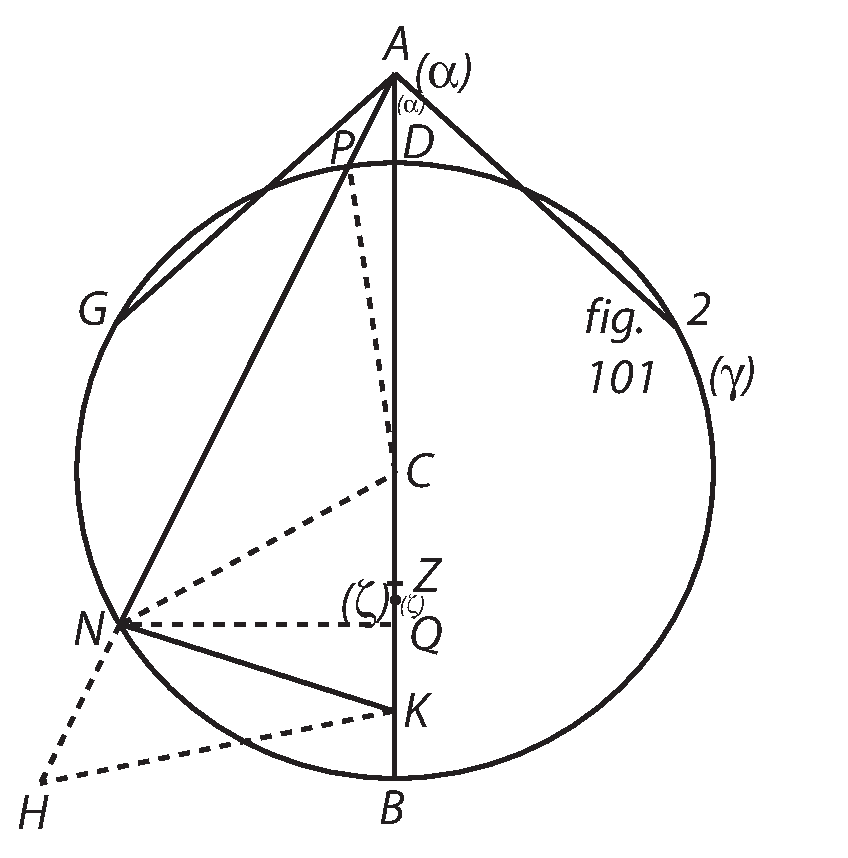
\includegraphics[width=0.4\textwidth]{images/T8_Barrow-2}
\end{center}
\clearpage
